%%%%%%%%%%%%%%%%%%%%%%%%%%%%%%%%%%%%%%%%%%%%%%%%%%%
%
%  New template code for TAMU Theses and Dissertations starting Fall 2012.  
%  For more info about this template or the 
%  TAMU LaTeX User's Group, see http://www.howdy.me/.
%
%  Author: Wendy Lynn Turner 
%	 Version 1.0 
%  Last updated 8/5/2012
%
%%%%%%%%%%%%%%%%%%%%%%%%%%%%%%%%%%%%%%%%%%%%%%%%%%%

%%%%%%%%%%%%%%%%%%%%%%%%%%%%%%%%%%%%%%%%%%%%%%%%%%%%%%%%%%%%%%%%%%%%%%
%%                           SECTION I
%%%%%%%%%%%%%%%%%%%%%%%%%%%%%%%%%%%%%%%%%%%%%%%%%%%%%%%%%%%%%%%%%%%%%


\pagestyle{plain} % No headers, just page numbers
\pagenumbering{arabic} % Arabic numerals
\setcounter{page}{1}


% \renewcommand*{\thefootnote}{\fnsymbol{footnote}}
\chapter[\uppercase{Introduction}]{\uppercase{Introduction}}
% \symbolfootnote[1]{Reprinted with permission from ``Introduction: The Importance of Research'' by AUTHOR et al., 2015. The Astrophysical Journal, Volume XYZ, Issue X, article id. XY, XY pp., Copyright 20XX by the American Astronomical Society.} }
% \renewcommand*{\thefootnote}{\arabic{footnote}}
% \setcounter{footnote}{0}

In this section we provide a basic introduction to some of the concepts used through this work. Specifically, we discuss what we mean by galaxy clusters, how they are used in cosmological measurements, how they are observed, current challenges with using their observations, the present constraints and the impact of this work.

\section{Galaxy Clusters}
Clusters of galaxies are the largest bound, highly over-dense, systems of galaxies which are held together by the cluster's own gravity. First recognized by 19th century astronomers, their place in astronomical canon was solidified when Edwin Hubble proofed their constituent nebulae where not bound to the Milky Way \citep{Hubble1926} but collections of stars similar to the Milky Way. Work to understand their nature and origin began in ernest when \cite{Hubble1931} used the virial theorem and the galaxy velocities in the centers of the Virgo \citep{Smith1936} and Coma \citep{Zwicky1933} clusters to derive their masses. The immense mass derived exceeded the total stellar mass contributed by all galaxies many times over. This lead Zwicky to theorize the existence of large amounts of non-luminous matter, and coining the term ``dark matter'' (DM), which we still use today.  

Some controversy surrounds what exactly constitutes a cluster. Traditionally, the richness \citep{Abell1958}, the number of galaxies above a certain brightness associated with the cluster, has defined the dividing line between rich clusters, and poor groups of galaxies. Clusters with a richness of 30 or more are traditionally referred to as clusters and those structures with richness between three and 30 are classified as groups. This definition is far from universal, and as such, in this work, we will not make such a distinction, any bound system of galaxies we refer to as a cluster.

\begin{figure}[ht]
	\begin{center}
		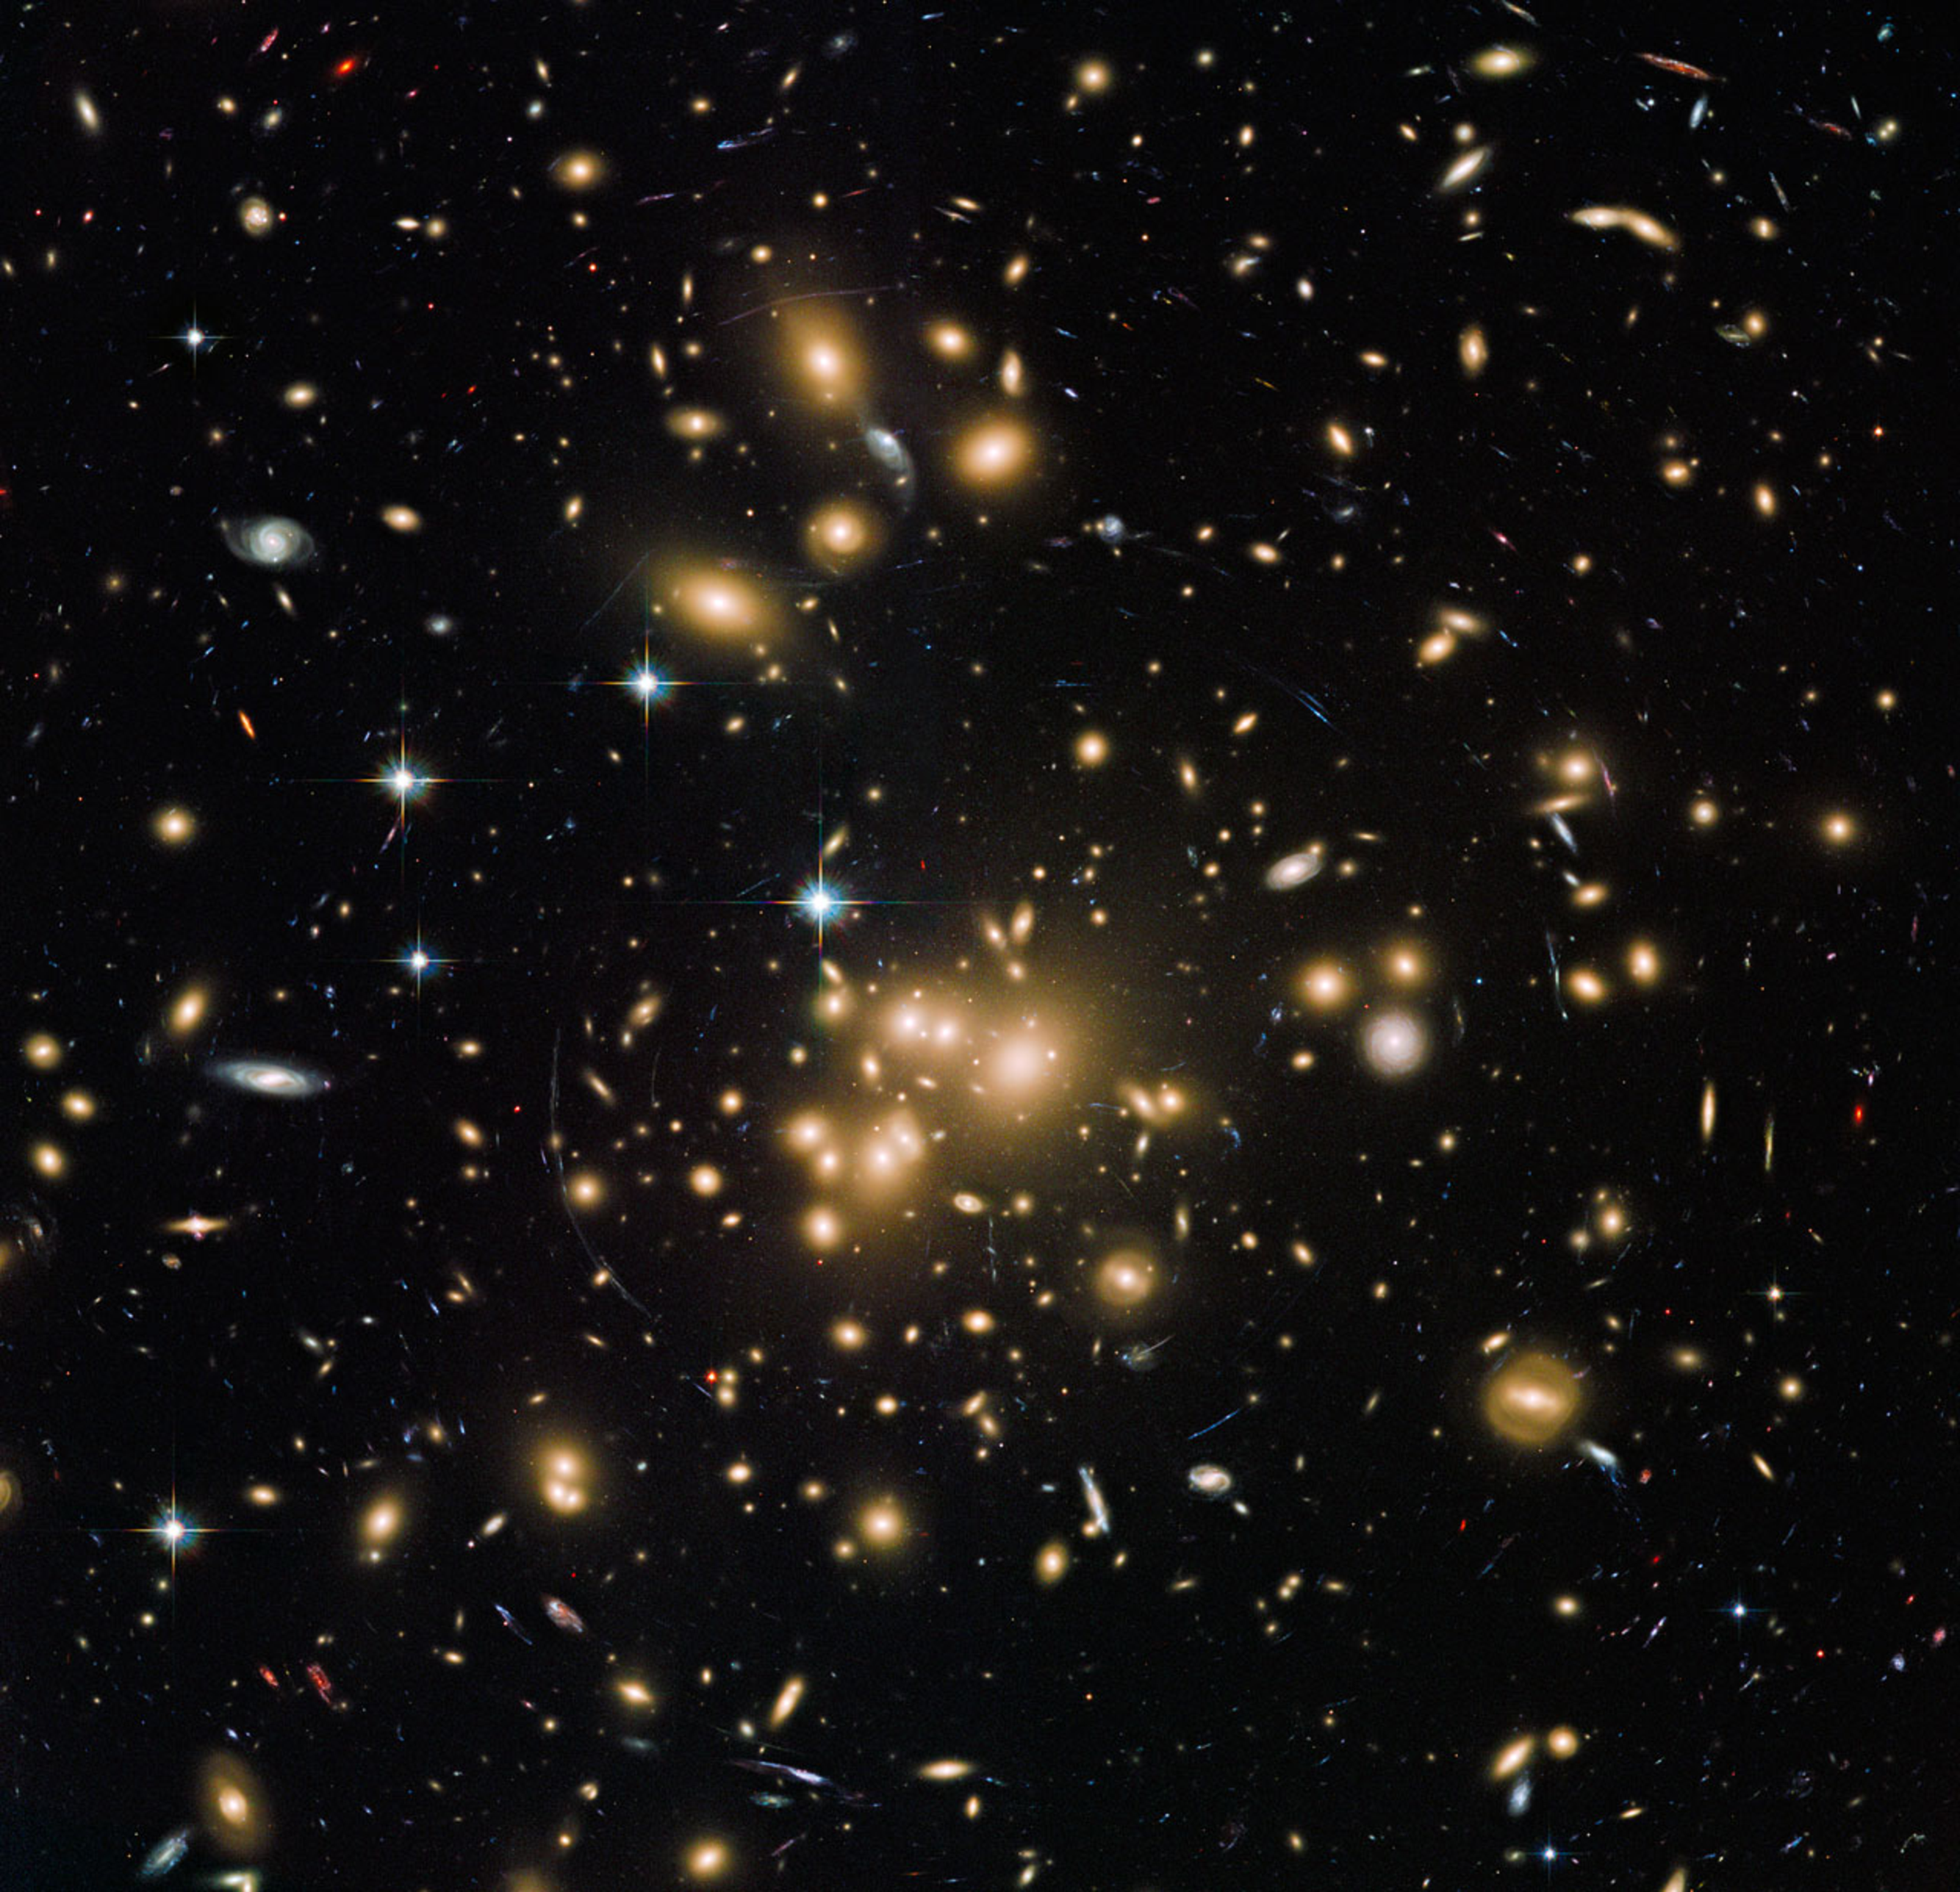
\includegraphics[width=0.6\textwidth]{figures/abell1689_hubble.pdf} 
	\end{center}
	\singlespace
	\caption{Hubble Space Telescope image of galaxy cluster Abell 1689.} Many of the galaxies visible are associated with the cluster. Not visible is the ICM or the larger DM halo which constitues the majority of the cluster mass.
	\label{fig: abell1689_hubble} 
\end{figure}

Modern astronomy gives the composition of galaxy clusters in three many parts. The galaxies themselves comprise the most obvious feature, and contain a large portion (but not the entirety) of the luminous matter (stars) in the cluster. The intracluster medium (ICM) is the space between the cluster galaxies and is composed many of ordinary matter (baryons) which are super heated to tens of thousands of kelvin. The ICM contains the bulk of the cluster's baryonic matter, and while it is very hot, it is not very dense, with a typical value of $10^{-3}$ particles per cubic centimeter. The majority of the cluster's mass is located in the DM halo which surrounds the cluster. For this reason, galaxy clusters are often referred to as halos, a term we use interchangeably throughout this work. Figure~\ref{fig: abell1689_hubble} shows a \emph{Hubble Space Telescope} Advanced Camera for Surveys image of galaxy cluster Abell 1689. Many of the cluster member galaxies have a similar yellow color. While the DM halo is not directly imaged, evidence for it can be seen by the very faint gravitational arcs of distant galaxies located behind the cluster.

Thought to form out of the primordial density fluctuations in the very early universe, the investigation of their formation and growth began in the 1960s. Soon thereafter, the hierarchical model of structure formation \citep{Press1974, Gott1975, White1978} was introduced. It suggests the first stars and stellar clumps grew then subsequently merged together with dark matter and other gas clumps to form the first galaxies which then continued to merge and grow into the clusters and large scale structures we see today. This accretion of smaller systems is thought to be driven by the gravity of the DM associated with the cluster. Of course, many complicated astrophysical processes are at work during cluster growth and similarly complicated theoretical models seek to explain these processes. For a detailed review of cluster formation see \cite{Kravtsov2012}.

Because their initial seeds were planted in the very early universe, the number and distribution of galaxy clusters across the sky is the finger print of the cosmology imprinted on the universe at its birth. To uncover the underlying cosmology a detailed understanding of the astrophysical processes that describe the motion of constituent galaxies and their impact on the ICM is required. So, galaxy clusters stand at the intersection of cosmology and astrophysics. 

\section{Cosmology with Galaxy Clusters}
The current concordance cosmology is a parametrization of the Big Bang cosmological model where the universe contains a cosmological constant ($\Lambda$; often referred to as dark energy) and cold dark matter (CDM). It is often characterized by six parameters; the Hubble Constant ($H_0$), the baryonic matter density ($\Omega_b$), the DM density ($\Omega_c$), the dark energy density ($\Omega_\Lambda$); the normalization of the power spectrum ($\sigma_8$); and the spectral index of the power spectrum ($n_s$). 

Galaxy clusters are sensitive probes of $\Omega_m$, the total mass ($\Omega_b + \Omega_c$) density in the universe and $\sigma_8$. Galaxy clusters trace the peaks in the universal matter density, often referred to as the power spectrum of matter density fluctuations or the matter power spectrum, much in the same way islands (mountain peaks) trace land masses through the ocean. We can constrain the values of $\Omega_m$ and $\sigma_8$ by comparing the number density of the observed galaxy clusters to that predicted by cosmological models.
 %Although, in reality, one measures $\sigma_8\Omega_m^\alpha$, where the value of $\alpha$ depends on the masses of the halos considered.

The determination of cosmological parameters is done by comparing the number of galaxy clusters per unit mass per unit comoving volume ($n(M,z)$) to models. See \cite{Allen2011} for a comprehensive review or \cite{Murray2013} for a more practical approach. $n(M,z)$, referred to as the halo mass function (HMF) captures the number evolution through a function which defines the particular model used. Early work by \cite{Press1974} and \cite{Bond1991} which assumed spherically symmetric halos, have largely been replaced by more modern fitting functions which, at the expense of an analytical solution, provide more accurate results when fit to simulation data. See \cite{Murray2013} for a review of the most common fitting functions used. Through this approach, the two parameters which clusters are most sensitive to, $\Omega_m$ and $\sigma_8$, are in reality measured as $\sigma_8\Omega_m^\alpha$, where the value of $\alpha$ depends on the masses of the halos considered. The degeneracy is broken through the evolution of the HMF as a function of redshift. 

% The $\Lambda$CDM model of cosmology makes explicit predictions about the number and masses of galaxy clusters throughout the universe. Connecting these predictions to a set of, sufficiently large in size, observed clusters remains a principal problem. Specifically, the largest threat to modern, precision, cluster cosmology is not the identification of large numbers of clusters (the total number of clusters known is only going up) but the accurate recovery of galaxy cluster mass. This problem extends to both the very rich clusters (those with high mass) and, importantly, the poor clusters (those with low mass) as the relationship between galaxy cluster mass and many of the observables which trace mass is not well understood for such low mass clusters.

\section{Observations of Galaxy Clusters}
In the coming years, many large surveys will add further statistical advantages to the determination of cosmological parameters using galaxy clusters. At their completion, the South Pole Telescope (SPT; \citealt{Carlstrom2011}) and the Atacama Cosmology Telescope (ACT; \citealt{Swetz2011}) are expected to find approximately one thousand clusters using observations in the millimeter combined with the SZ effect. Attempts are already underway to calibrate these observations using subsamples of clusters (approximately 100 cluster candidates and 60 clusters respectively) and other observables such as virial estimates or X-ray temperature measurements \citeeg{Sifon2013, Bocquet2015}. 

X-ray identified clusters, up until today, have mostly been observed fortuitously through targeted \textit{Chandra} or \textit{XMM-Newton} observations. That is soon to change with the \textit{eROSITA} telescope onboard the Spektrum-Roentgen-Gamma Mission, which will perform an all--sky survey during its four year mission and detect an estimated 50,000 or more clusters.

Large optical surveys such as the Dark Energy Survey (DES; \citealt{DES2005}) and the Large Synoptic Survey Telescope (LSST) will survey enormous portions of the sky extremely deeply and will identify vast numbers of clusters using optical selection methods \citeeg{Rykoff2014, Rozo2014}. However, the majority of these surveys will be photometric, and any spectral information will be obtained from preexisting datasets. And while it is possible to estimate cluster masses using photometric redshifts, primarily through the richness--mass relation, \citeeg{Rykoff2012, Rykoff2014}, spectroscopic followup is required to both better calibrate the relation and to obtain the level of precision needed to compete with other mass estimators. 

\section{Galaxy Cluster Surveys as a Data Science Challenge}
Astronomy and astrophysics are undergoing a data revolution. The advances in telescope design, detectors, and computing resources have provided more astronomical data than any previous time in the history of the field. Beginning in the early 2000s, astronomical surveys have generated many hundreds of terabytes of data for many millions of sources. In the coming years, this data excess will grow beyond the terabyte regime with observations of billions of astronomical objects. And, galaxy clusters certainly makeup a portion of those observations. 

50,000 or more X-ray identified clusters will be found by the upcoming eROSITA telescope onboard the \emph{Spektrum-Roentgen-Gamma} Mission. The South Pole Telescope and the Atacama Cosmology Telescope are discovering many thousands of clusters through the Sunyaev-Zel’dovich Effect (SZE). The Dark Energy Survey (DES) and planned Large Synoptic Survey Telescope (LSST) will optically identify \citeeg{Rykoff2014} many tens of thousands of clusters with much lower masses than is possible with SZE measurements. The data products from these surveys will be both immense and heterogeneous. The number of data ``features'' associated with each cluster can be many tens. The different observation wavelengths probe different cluster physics making them more or less sensitive. The instruments used to collect the data have varying angular resolutions, owing from both the wavelengths observed and ground versus space based observations. Therefore, the combination of datasets will be a significant challenge.

\subsection{Machine Learning}
Machine learning (ML) is a branch of computer science focused on the study and construction of computational tools which can learn from and make predictions based on data. In 1959, Arthur Samuel (December 5, 1901 -- July 29, 1990), an early computer gaming pioneer, described ML as a ``Field of study that gives computers the ability to learn without being explicitly programmed.'' While, a great deal of programming is often required (discussed further below), such algorithms work by comparing data to a set of models allowing them to make predictions based on the data rather than preprogrammed commands.

ML can be broken into two large categories. ``Unsupervised learning'' where the ML is tasked to make qualitative statements about the data which were not previously known. An example would be finding clusters of data inside a large dataset, where the number and location of the clusters are not known a priori (\eg, locating galaxy clusters in observations of galaxy positions). ``Supervised learning'' asks the computer to make predictive statements about one variable based on the observations of another or combination of variables. An example could be photometric redshift prediction. Given a large number of color and magnitude measurements for a galaxy, predict the most probable redshift.  

In this work, we are concerned with supervised learning, where we know a relationship exists between two sets of data, and we use a computer algorithm to infer the relationship for us. To do this learning, we use an algorithm called decision tree learning which works by mapping a set of observations (``features'' in ML speak) of an source to a set of conclusions (``targets'') about that source. If the set of conclusions is finite then the method becomes a classification tree, and if the conclusions infinite then it becomes a regression tree. 

\begin{figure}[ht]
	\begin{center}
		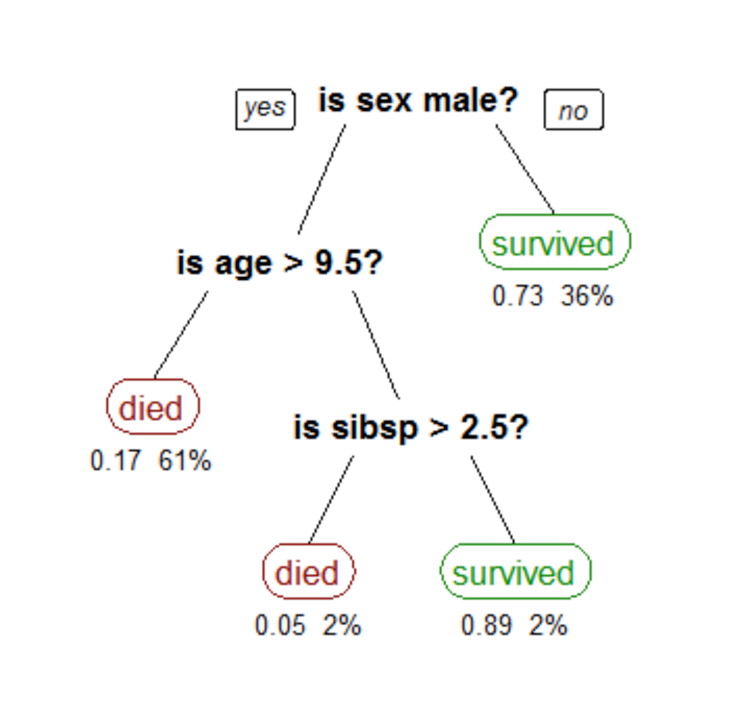
\includegraphics[width=0.6\textwidth]{figures/CART_tree_titanic_survivors.pdf} 
	\end{center}
	\caption{An example of a classification tree.}
	Decision tree classifying the survival of passengers on the RMS Titanic. ``sibsp'' represents the number siblings or spouses aboard, and the numbers below each class represents the probability of survival and fraction of passengers which are classified into each leaf. 
	\label{fig: cart tree} 
\end{figure}

Figure~\ref{fig: cart tree}\footnote{By Stephen Milborrow (Own work) [CC BY-SA 3.0 (http://creativecommons.org/licenses/by-sa/3.0) or GFDL (http://www.gnu.org/copyleft/fdl.html)], via Wikimedia Commons} shows a simple example of a classification tree for the survivability of passengers on the RMS Titanic. The bolded text are referred to as interior nodes which correspond to a single feature of each passenger in the example, sex, age and number of siblings or spouses. The ending points are called leaves which represents the value of the target variable given the value of the features input into the tree. For this example, there are two possible ending leaves, ``died'' or ``survived.'' Using this simple tree we are able to classify all passangers into the two possible classes. 

The ML algorithm ``learns'' this tree by choosing a feature from all available features which best splits the input data into two or more subsets. In the case of the example this is the sex of the passenger. This becomes the root node. All subsequent nodes are created by repeating this process on each subset associated with the previous node. So, it will split the male passengers by age, and then by number of siblings for the males older than 9.5 years. This process is known as a top-down induction of decision trees and is the most common method for creating decision trees from data.

Once the decision tree has been learned it can be used to classify data it has not seen before. For example, a 30 year-old, male passenger of the RMS Titanic has a probability of survival of 17\% and so will most likely be classified as ``died'' by the ML algorithm. However, imagine for a moment, with the benefit of hindsight that we know this male passenger survives. Only 17\% of the time will the ML method classify the passneger as ``survived'' based on this decision tree. We can boost the predictive power of the tree by generating many trees, and then combining the final predictions at the end. Methods that construct more than one tree are called ensemble methods. For this work, we use an ensemble method know as a forest of randomized trees, and discuss them more in Sections \editorial{XXXX}.

\section{State of Play}
As mass is not a direct observable, a lot of work is underway to characterize galaxy cluster masses with an observable feature of galaxy clusters. In this section, we will briefly touch on a few of the ways cluster mass is determined, and address any short comings the method may have. Generally, the methods fall into two distinct camps, simulation based and direct or statistical calibration. The goal is to constrain, as best possible, $P(X|M,z)$ or the probability ($P$) that a galaxy cluster of given mass ($M$) located at redshift ($z$) using observable parameter ($X$).

One could use various simulations to attempt to calibrate this observable--mass relation \citeeg{Vanderlinde2010, Sehgal2011}. However, the primary challenge to this method is the incomplete understanding of the baryonic physics which take place in galaxy cluster environments. While there have been (and continue to be) many improvements in the accuracy and power of simulations it is doubtful that in the coming years they will reach the accuracy level required to the point where the observable--mass relation is dominated only by statistics \citep{Weinberg2013}. 
 
The second broad camp is the direct calibration of cluster masses. This recipe has two distinct but not always independent tracks. The ``direct'' method uses the direct observations of a small set of clusters and then uses known mass estimators, X-ray hydrostatic or weak lensing (WL) as examples, which provide a ``true'' mass. This directly calibrates the observable--mass relation which is then applied to a much larger sample. The complications lie in that the ``true'' masses are in fact estimations, and the methods used to recover these masses are subject to their own limitations. X-ray hydrostatic estimations assume hydrostatic equilibrium \citeeg{Mantz2015} which may only be valid for a very small number and range of cluster masses. The Sunyaev--Zel’dovich (SZ; \citealt{Sunyaev1972}) effect, which uses the up--scattering of cosmic microwave background (CMB) photons to estimate cluster masses, provides accurate estimations of mass, but the ability to detect low mass galaxy clusters is currently limited by technology \citeeg{Carlstrom2002a}. WL estimates are, in principle, correct in the mean, but they suffer from signal-to-noise requirements, limiting their usefulness in low mass clusters, and potentially suffer from line-of-sight effects as the effect is sensitive to all mass along the line of sight. Virial mass estimators which determine the cluster mass based on the motions of the member galaxies is promising in that it is a direct measurement of the depth of clusters potential well, but suffers from systematics due to cluster formation physics which disrupts the velocity field.
 
The statistical method of determining galaxy cluster mass relies not on direct measurements of individual clusters but the calibration of observables for the entire sample which correlate with cluster mass. One example is the spatial clustering of the galaxy clusters themselves. See \cite{Weinberg2013} for a comprehensive review. In practice, it will be a combination of the three methods touched on that will provide the most reliable determination of cluster masses. 

Virial mass estimators, specifically, can be applied in both a direct and statistical fashion. Currently, the accuracy of such a method, especially to the level required for today's precision cosmology, is not well constrained. In the coming years large spectroscopic surveys will provide enough coverage, and so these methods warrant further investigation \citeeg{Saro2013}.

\section{This Work}
As the sample of known clusters grows to many tens of thousands, spectroscopic followup becomes unfeasible. Large spectroscopic surveys will be required to reduce systematics to a level that will allow accurate mass estimations using virial methods. The Hobby Eberly Dark Energy Experiment (HETDEX; \citealt{Hill2008}) is a forthcoming blind spectroscopic survey that could potentially be used to accurately calibrate the observable-mass relation for a significant number of galaxy clusters at both extremes of the mass scale. HETDEX is designed to measure the dark energy equation of state at $z\sim2$, and so the applicability to galaxy cluster science has not yet been investigated.

Given how much progress could be made with HETDEX, this work seeks to address this issue in two ways. First, using a set of state-of-the-art simulations we will simulate the observing strategy of HETDEX to determine the number and nature of clusters that might be observed. See Section. This is done in four distinct ways and in each part we will measure the dynamical properties, such as redshift, LOSVD, and mass of the clusters. First we will use targeted observations and perfect knowledge of the observed galaxy clusters, which includes center, membership, and number to recover the desired properties. Secondly, we will assume that we know the location but not the center, membership, or number of constituent galaxies. Then we will employ the HETDEX observing strategy, including realistic pointing pattern, observational magnitude constraints, and spectral sensitivity limits to generate a set of realistic observations which are then used with perfect and less than perfect knowledge scenarios to determine the cluster properties. 

In all cases, we will attempt to characterize the observable--mass relation (or relations) to better understand the dominate sources of uncertainty when using HETDEX like observations. This will enable us to more fully understand and constrain the HMF which, in turns, allows us to make more accurate measurements of the cosmological parameters traced by galaxy clusters.

The second effort of this work, outlined in Section, will use targeted spectroscopic observations of ten nearby clusters with the Mitchell Spectrograph (formerly known as VIRUS-P; \citealt{Hill2008a}), an integral field unit (IFU) in a square array of 246 $4.24''$ diameter optical fibers, to test some of the methods used in the first method. This will provide insight in how the observable--mass relation may be improved through followup observations of targeted clusters.
